\documentclass[journal]{IEEEtran}


\usepackage[utf8]{inputenc}
\usepackage{graphicx}
\usepackage{amsmath}
\usepackage{amsthm}
\usepackage{amssymb}
\usepackage{hyperref}
\usepackage{subfig}
\usepackage{multirow}
\usepackage[section]{placeins}


% correct bad hyphenation here
\hyphenation{op-tical net-works semi-conduc-tor}


\begin{document}
%
% paper title
% Titles are generally capitalized except for words such as a, an, and, as,
% at, but, by, for, in, nor, of, on, or, the, to and up, which are usually
% not capitalized unless they are the first or last word of the title.
% Linebreaks \\ can be used within to get better formatting as desired.
% Do not put math or special symbols in the title.
\title{Vehicle Driving Assistant}
%
%
% author names and IEEE memberships
% note positions of commas and nonbreaking spaces ( ~ ) LaTeX will not break
% a structure at a ~ so this keeps an author's name from being broken across
% two lines.
% use \thanks{} to gain access to the first footnote area
% a separate \thanks must be used for each paragraph as LaTeX2e's \thanks
% was not built to handle multiple paragraphs
%

\author{Akanksha~Dwivedi,
        Anoop~Toffy,
        Athul~Suresh,
        and~Tarini~Chandrashekhar,~\IEEEmembership{International Institute of Information Technology, Bangalore}}% <-this % stops a space


% note the % following the last \IEEEmembership and also \thanks - 
% these prevent an unwanted space from occurring between the last author name
% and the end of the author line. i.e., if you had this:
% 
% \author{....lastname \thanks{...} \thanks{...} }
%                     ^------------^------------^----Do not want these spaces!
%
% a space would be appended to the last name and could cause every name on that
% line to be shifted left slightly. This is one of those "LaTeX things". For
% instance, "\textbf{A} \textbf{B}" will typeset as "A B" not "AB". To get
% "AB" then you have to do: "\textbf{A}\textbf{B}"
% \thanks is no different in this regard, so shield the last } of each \thanks
% that ends a line with a % and do not let a space in before the next \thanks.
% Spaces after \IEEEmembership other than the last one are OK (and needed) as
% you are supposed to have spaces between the names. For what it is worth,
% this is a minor point as most people would not even notice if the said evil
% space somehow managed to creep in.



% The paper headers
\markboth{Project Report, \today}%
{Shell \MakeLowercase{\textit{et al.}}: Bare Demo of IEEEtran.cls for IEEE Journals}
% The only time the second header will appear is for the odd numbered pages
% after the title page when using the twoside option.
% 
% *** Note that you probably will NOT want to include the author's ***
% *** name in the headers of peer review papers.                   ***
% You can use \ifCLASSOPTIONpeerreview for conditional compilation here if
% you desire.

% use for special paper notices
\IEEEspecialpapernotice{(Draft Paper)}

% make the title area
\maketitle

% As a general rule, do not put math, special symbols or citations
% in the abstract or keywords.
\begin{abstract}
Autonomous vehicles has been a common term in our day to day life with
car manufacturers like Tesla shipping cars that are SAE Level 3. While
these vehicles include a slew of features such as parking assistance and cruise
control, they’ve mostly been tailored to foreign roads. Potholes, and the
abundance of them, is something that is unique to our Indian roads. We
believe that successful detection of potholes from visual images can be applied
in a variety of scenarios. Moreover, the sheer variety in the color, shape and
size of potholes makes this problem an apt candidate to be solved using
modern machine learning and image processing techniques.
\end{abstract}

% Note that keywords are not normally used for peerreview papers.
\begin{IEEEkeywords}
Image processing, Machine Learning, Pot hole detection, Clustering
\end{IEEEkeywords}

\IEEEpeerreviewmaketitle



\section{Introduction}
The project aims to provide a comprehensive set of assistance features to aid the driver (or autonomous vehicle) to drive safely. This could includes a number of indicators about the environment, the major cue being visualisation and detection of potholes in the road ahead. 

"A pothole \cite{pothole} is a structural failure in a road surface, caused by failure primarily in asphalt pavement due to the presence of water in the underlying soil structure and the presence of traffic passing over the affected area". An example of a road with pothole is shown in Figure 1.

\begin{figure}[!h]
\begin{center}
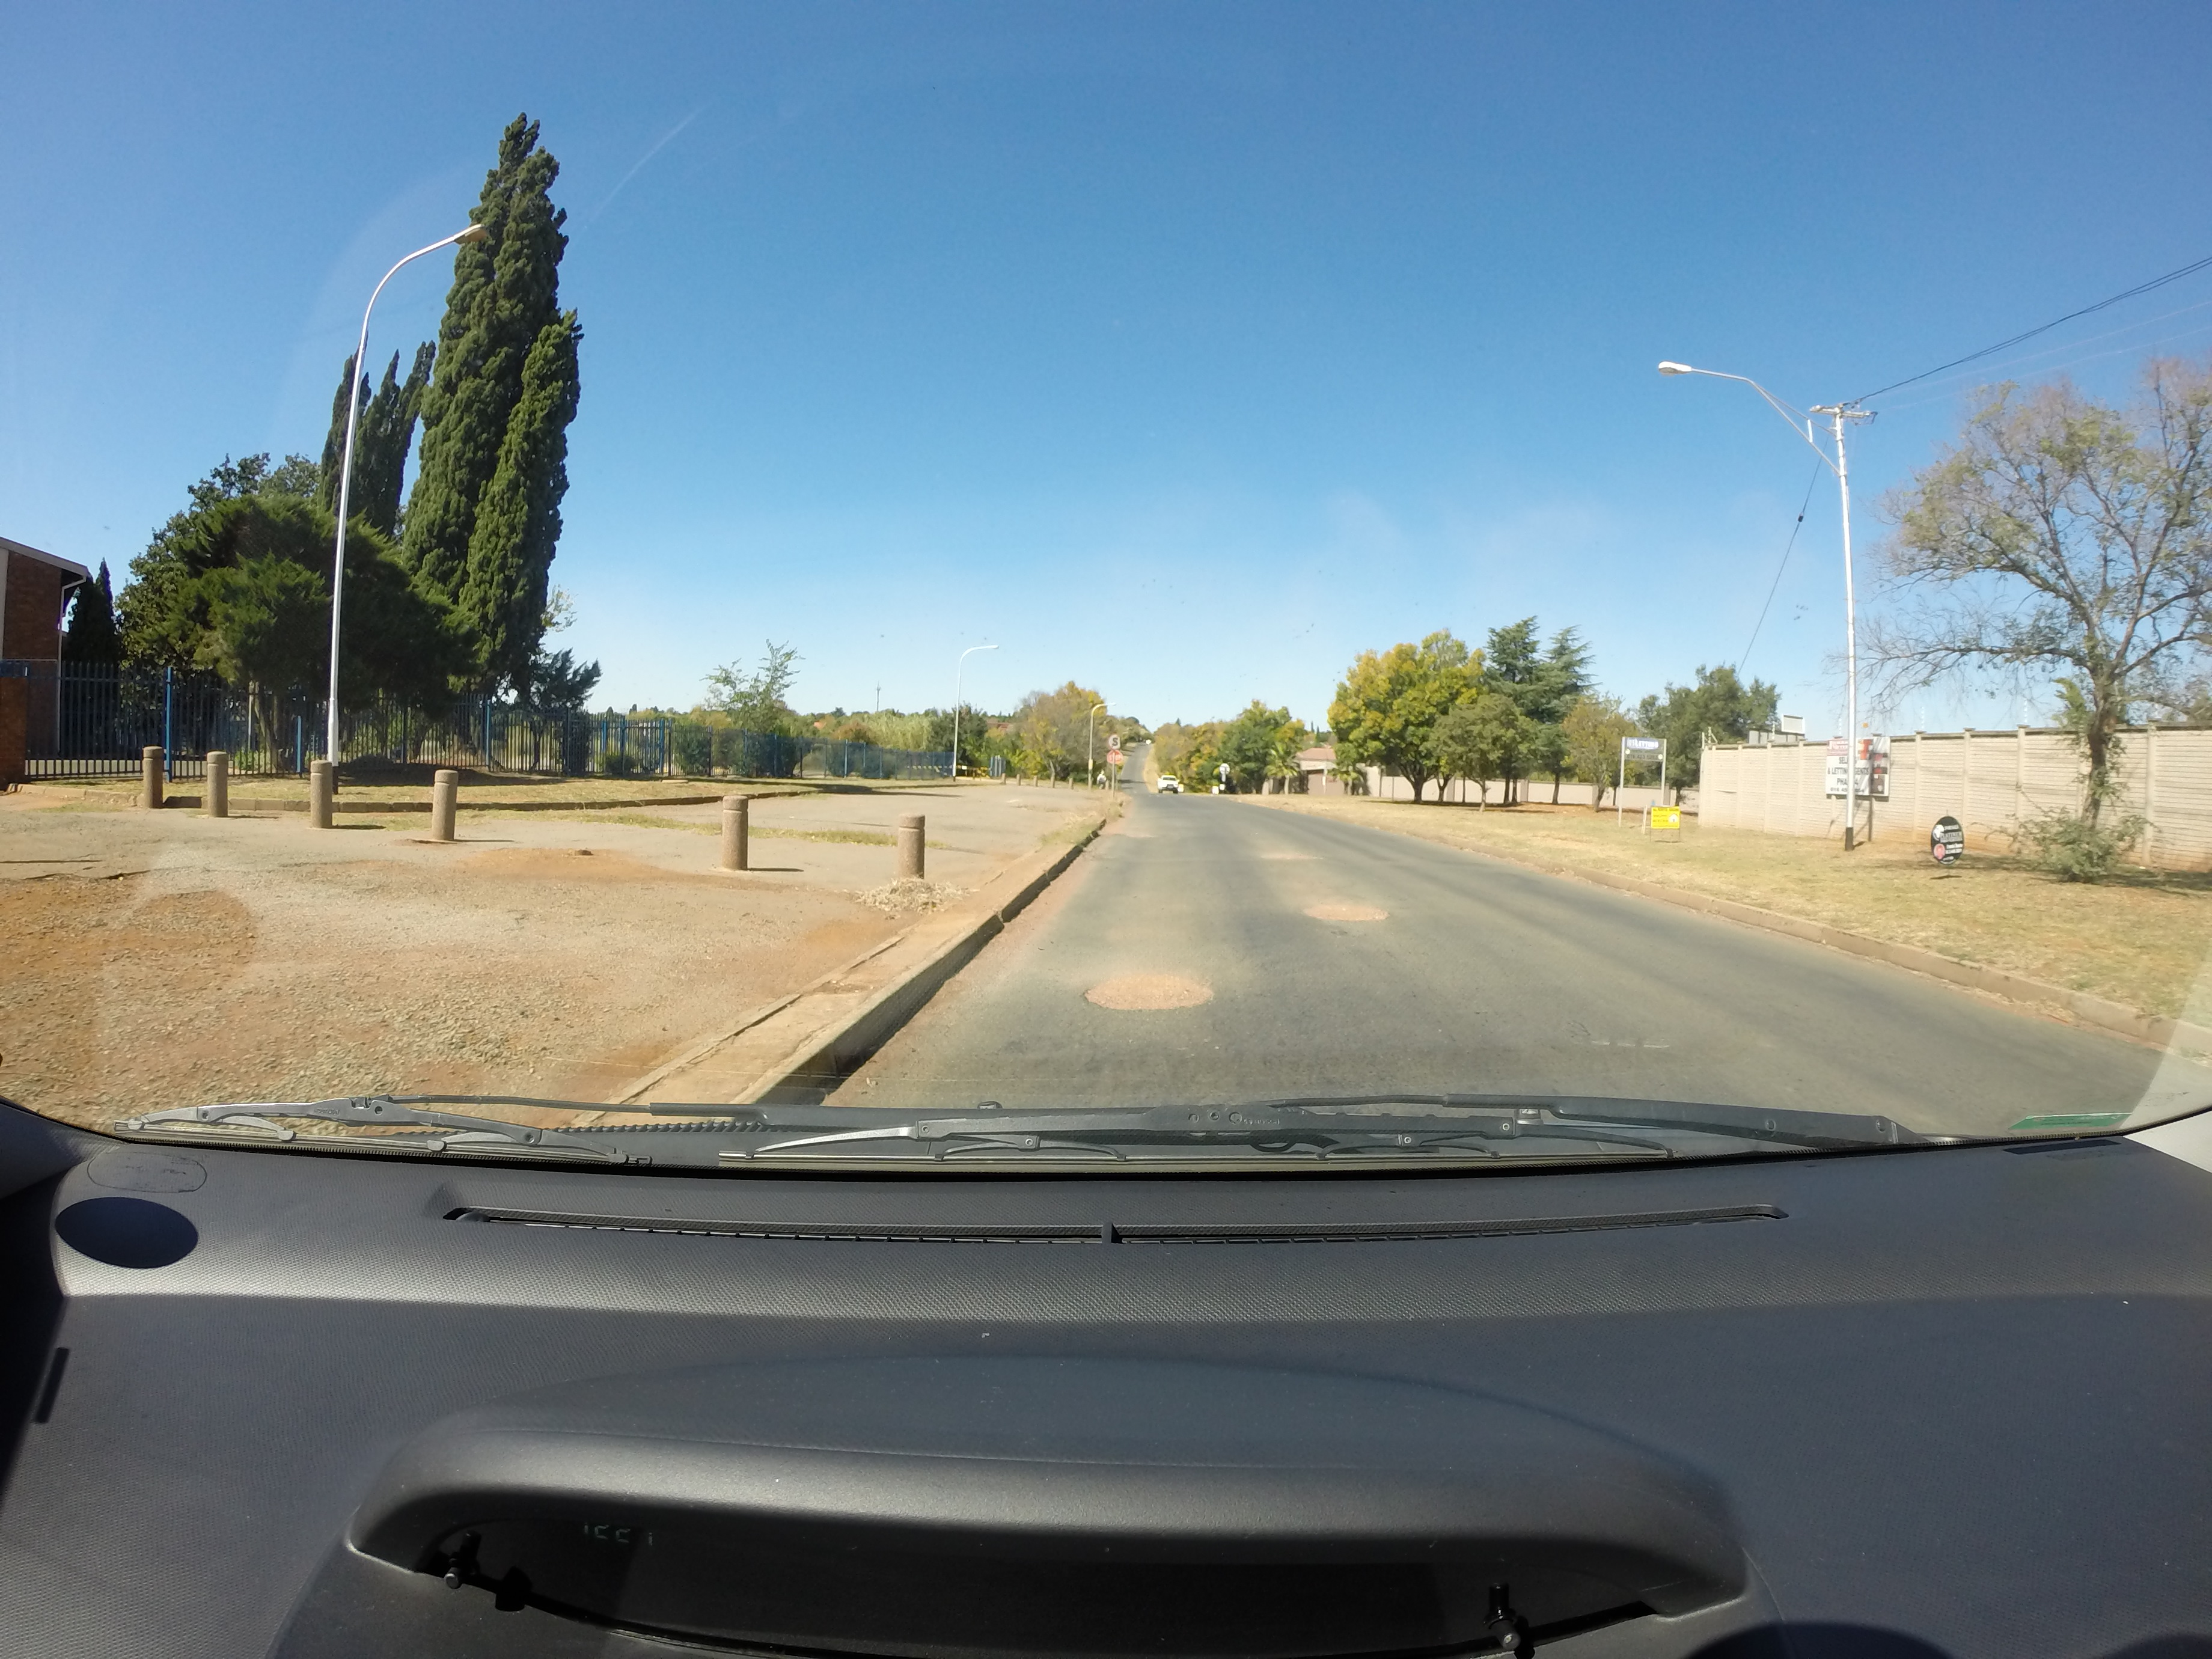
\includegraphics[scale=0.035]{Images/pothole_example.JPG}
\end{center}
\caption{Pothole example}
\end{figure}

The remainder of the paper is structured as follows. We present a brief history of the related work done so far in the field of pothole detection and visualisation in Section 2. Section 3 discusses about the experimental set up we used in this work.In the subsequent section we describes the methodology that we follow in the following section 4. It includes road extraction part and blob detection part. Then the result that we obtained are given briefly in section 5. Finally section 6 concludes the paper.
% You must have at least 2 lines in the paragraph with the drop letter
% (should never be an issue)

\section{Related Work}
In Nienaber et al (2015) \cite{paperone}, a system using basic image processing techniques in a constrained environment without relying on any machine learning techniques is used for pothole detection. It presents a good preliminary method for detecting potholes using a single camera within an range of 2 - 20m from a vehicle moving at a speed of not more than 60km/hr. The method separates a rectangular area of interest just above the hood of the vehicle which contains road surface, assuming that driver maintains a safe distance from the front vehicle. The rectangular area of interest is separated by connecting the various farthest region of interest using convex hull algorithm.

\vspace*{.5cm}

The work presented by Ajit Danti et al (2012) \cite{papertwo}, presents a comprehensive approach to address the acute problems of Indian roads such as faded lanes, irregular potholes, improper and invisible road signs. Instead of using image processing techniques for pothole detection as done by Nienaber et al (2015), Ajith Danti et al (2012) uses K-Means clustering based algorithm to detect potholes. By addressing the acute problems above mentioned in the paper it makes automated driving safer and easier in Indian roads. 

\section{Proposed Work}
In this paper we use both image processing techniques as well as machine learning to study the presence and occurrence of potholes. At first we used a Digital camera mounted on the window of a slow moving vehicle to capture the potholes images. The images are captured at high resolution so that the analysis of the potholes will be easier. This paper propose a way to visualize the potholes as well as identify whether or not the road has a pothole in it. The visualisation approach is similar to how humans perceive the pothole images in the brain. The pothole identification approach will help to signal the driver of a vehicle to take preventive actions upon pothole infected lanes.

For visualising the pothole we first extract a region of the interest from the given image which will contain the road area. Since extracting the road area will help to narrow down the area of interest. This way we will be able to prevent the irrelevant informations from the analysis like foliage, vehicle hood, other vehicles on the road etc. We then apply image processing techniques like contour detection, blob detection and edge detection to draw a bounding box over the area of the road which contains the potholes.

For machine learning technique we use annotated dataset \cite{dataset} for training various classifiers and then try various machine learning algorithms to figure out the presence of a pothole in the frame given.

\section{Methodology}

In this section we briefly familiarize the methodology that we used for the visualisation and detection of potholes in detail. The subsequent section first discusses about the image processing techniques that are helpful for pothole visualisation followed by feature extraction and machine learning learning techniques  used in the study.

\subsection{Image Processing Techniques}

\subsubsection{Road Extraction Method}

The figure 2 show the image that we collected from the Digital camera. The image is then converted to its corresponding HSV channel because we found out the HSV channels are good for analysing the image with various image processing techniques. 

\begin{figure}[!htb]
\begin{center}
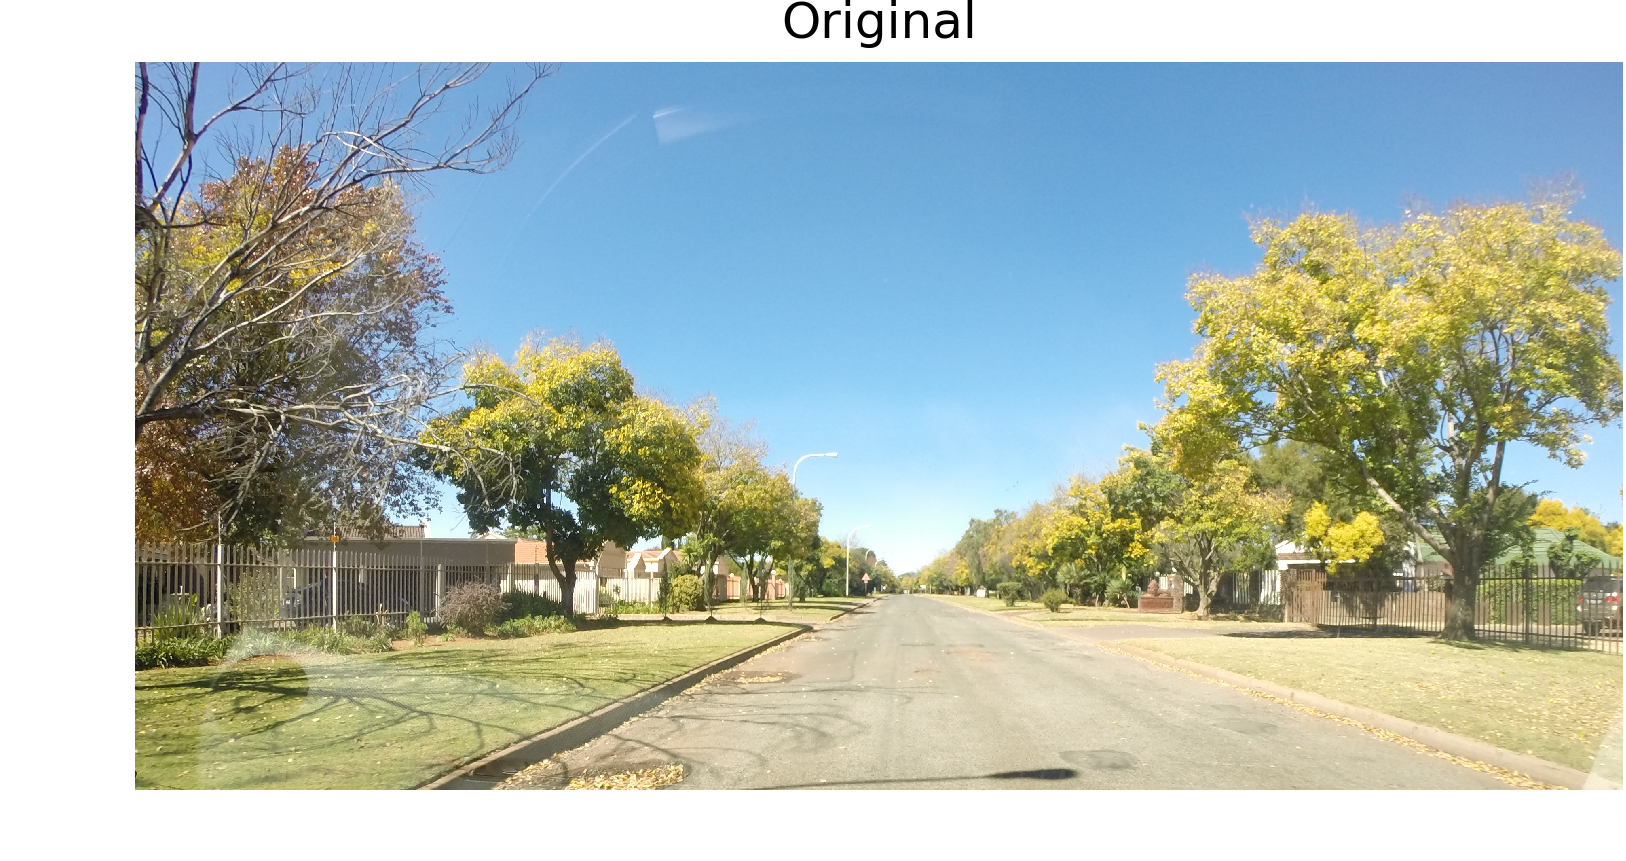
\includegraphics[scale=0.25]{Images/0_Original.png}
\end{center}
\caption{Pothole Image}
\end{figure}


\begin{figure}[!htb]
\begin{center}
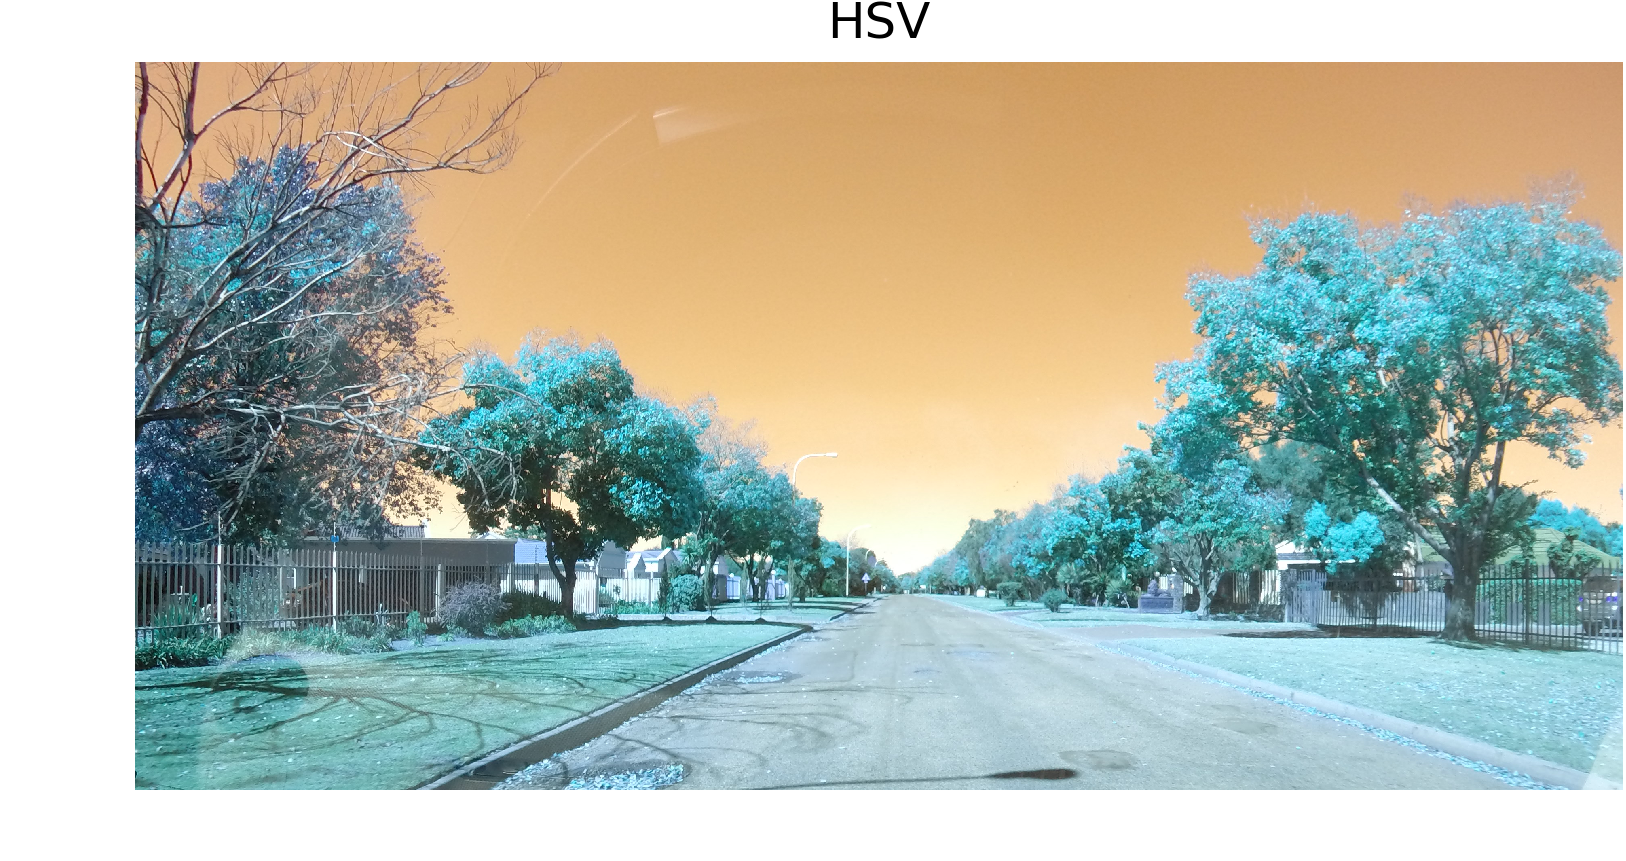
\includegraphics[scale=0.25]{Images/1_HSV.png}
\end{center}
\caption{Converting to HSV}
\end{figure}

From the 
\begin{figure}[!htb]
\begin{center}
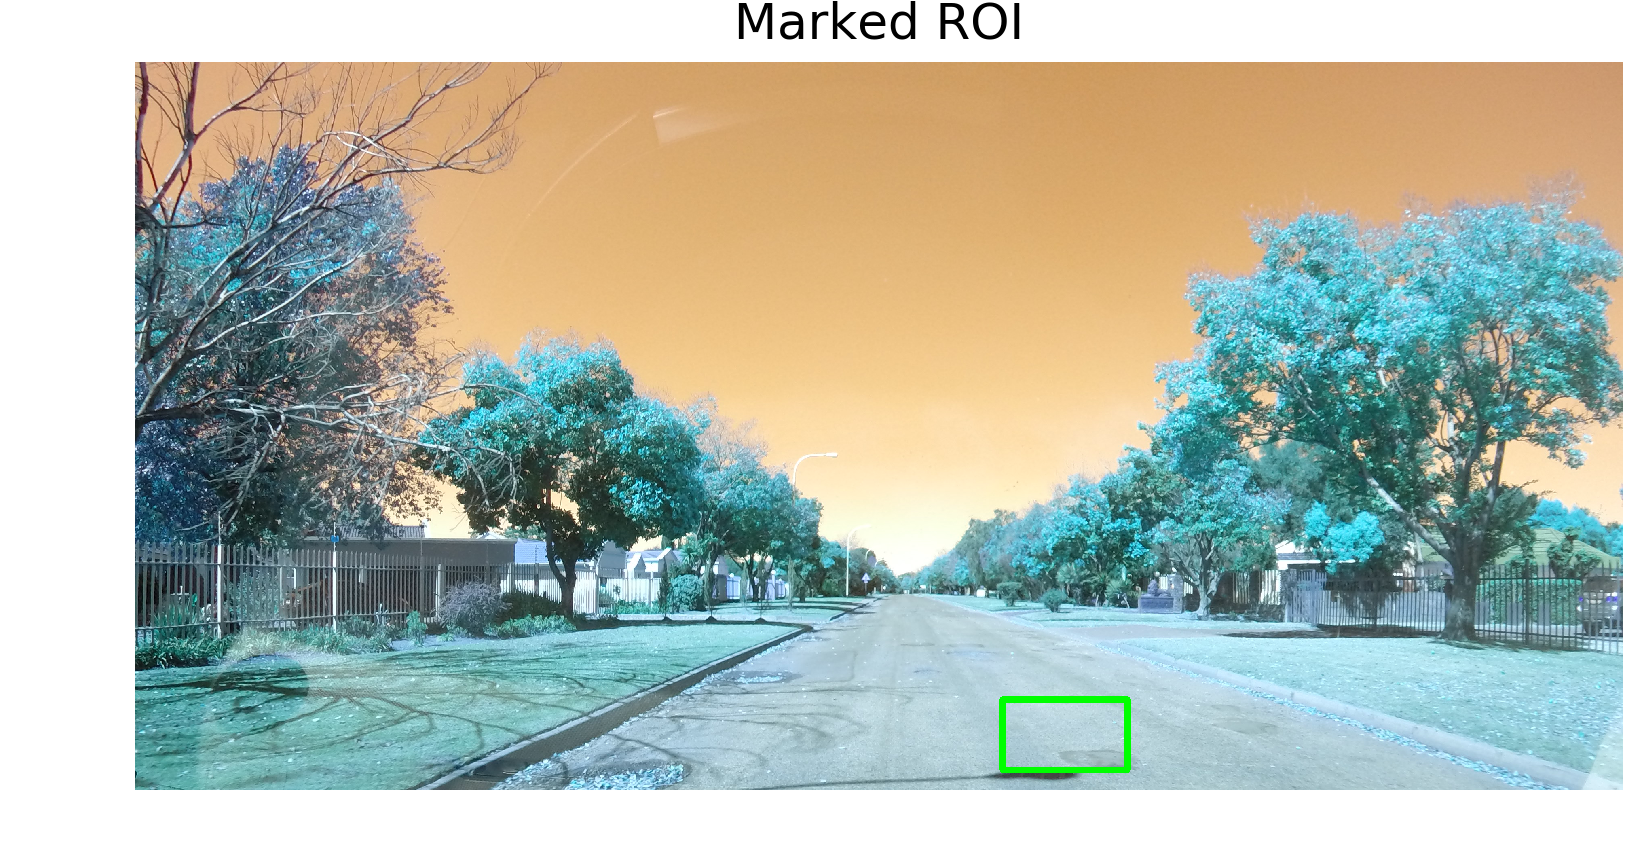
\includegraphics[scale=0.25]{Images/2_Marked_ROI.png}
\end{center}
\caption{Selecting the ROI}
\end{figure}

\begin{figure}[!htb]
\begin{center}
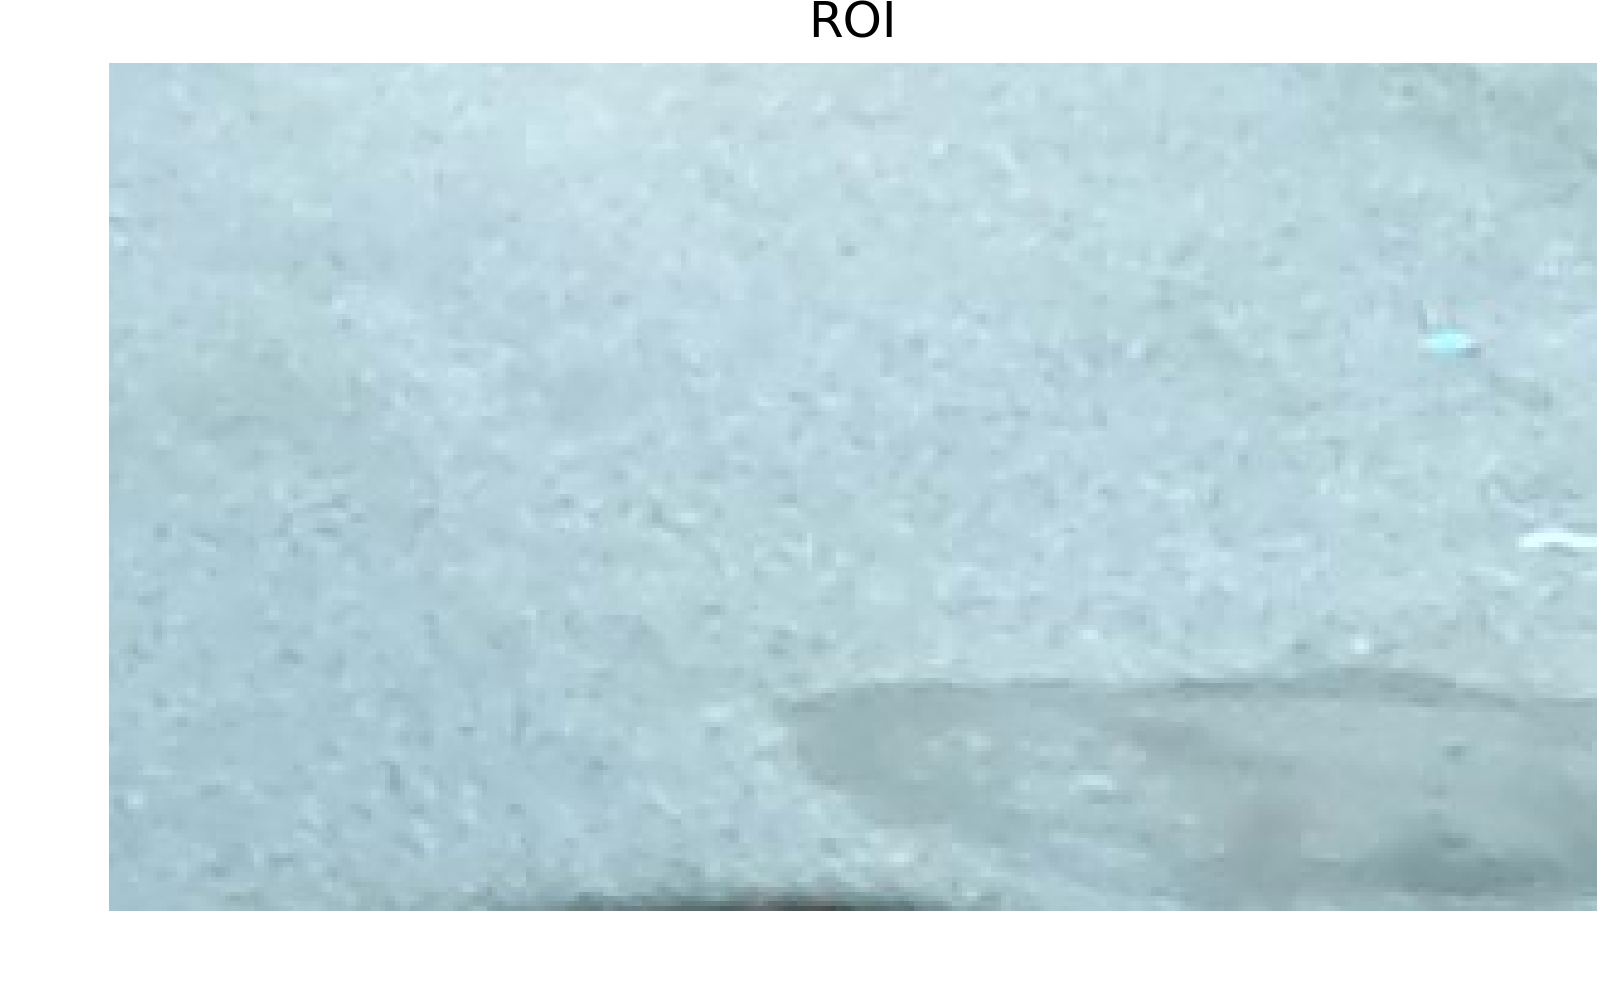
\includegraphics[scale=0.25]{Images/3_ROI.png}
\end{center}
\caption{Region of Interest}
\end{figure}

\begin{figure}[!htb]
\begin{center}
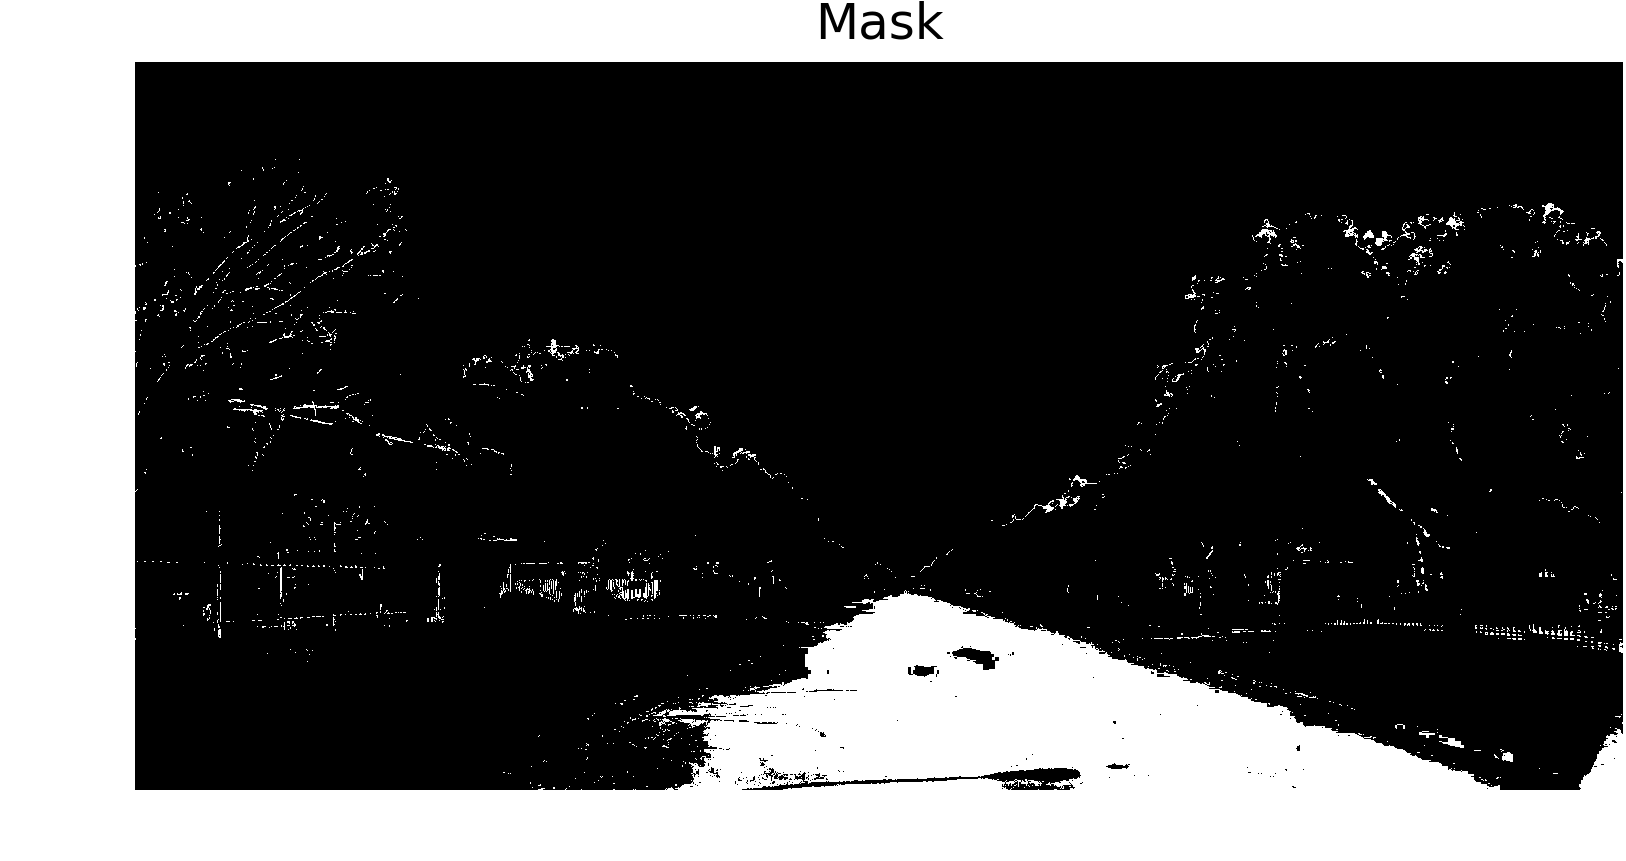
\includegraphics[scale=0.25]{Images/4_Mask.png}
\end{center}
\caption{Mask}
\end{figure}


\begin{figure}[!htb]
\begin{center}
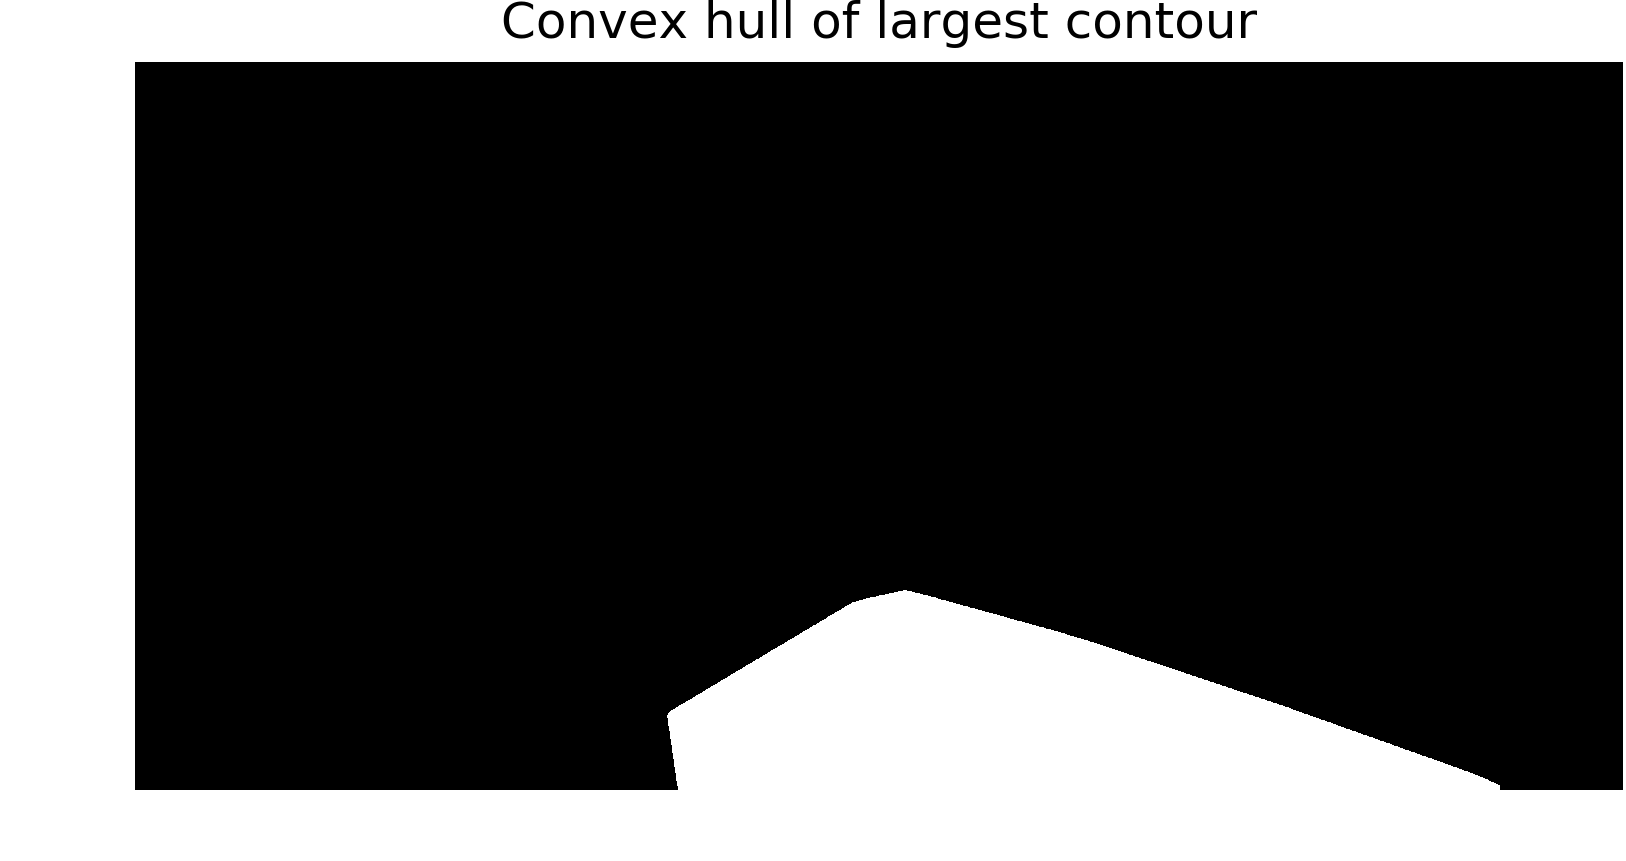
\includegraphics[scale=0.25]{Images/5_Convex_hull_of_largest_contour.png}
\end{center}
\caption{Convex hull of largest contour}
\end{figure}


\begin{figure}[!htb]
\begin{center}
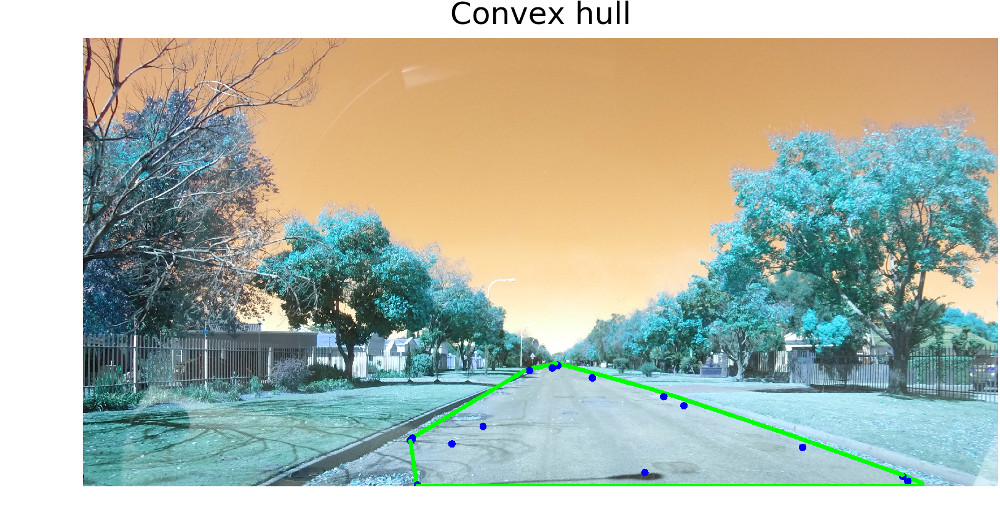
\includegraphics[scale=0.25]{Images/6_Convex_hull.png}
\end{center}
\caption{Convex hull on Original Image}
\end{figure}


\begin{figure}[!htb]
\begin{center}
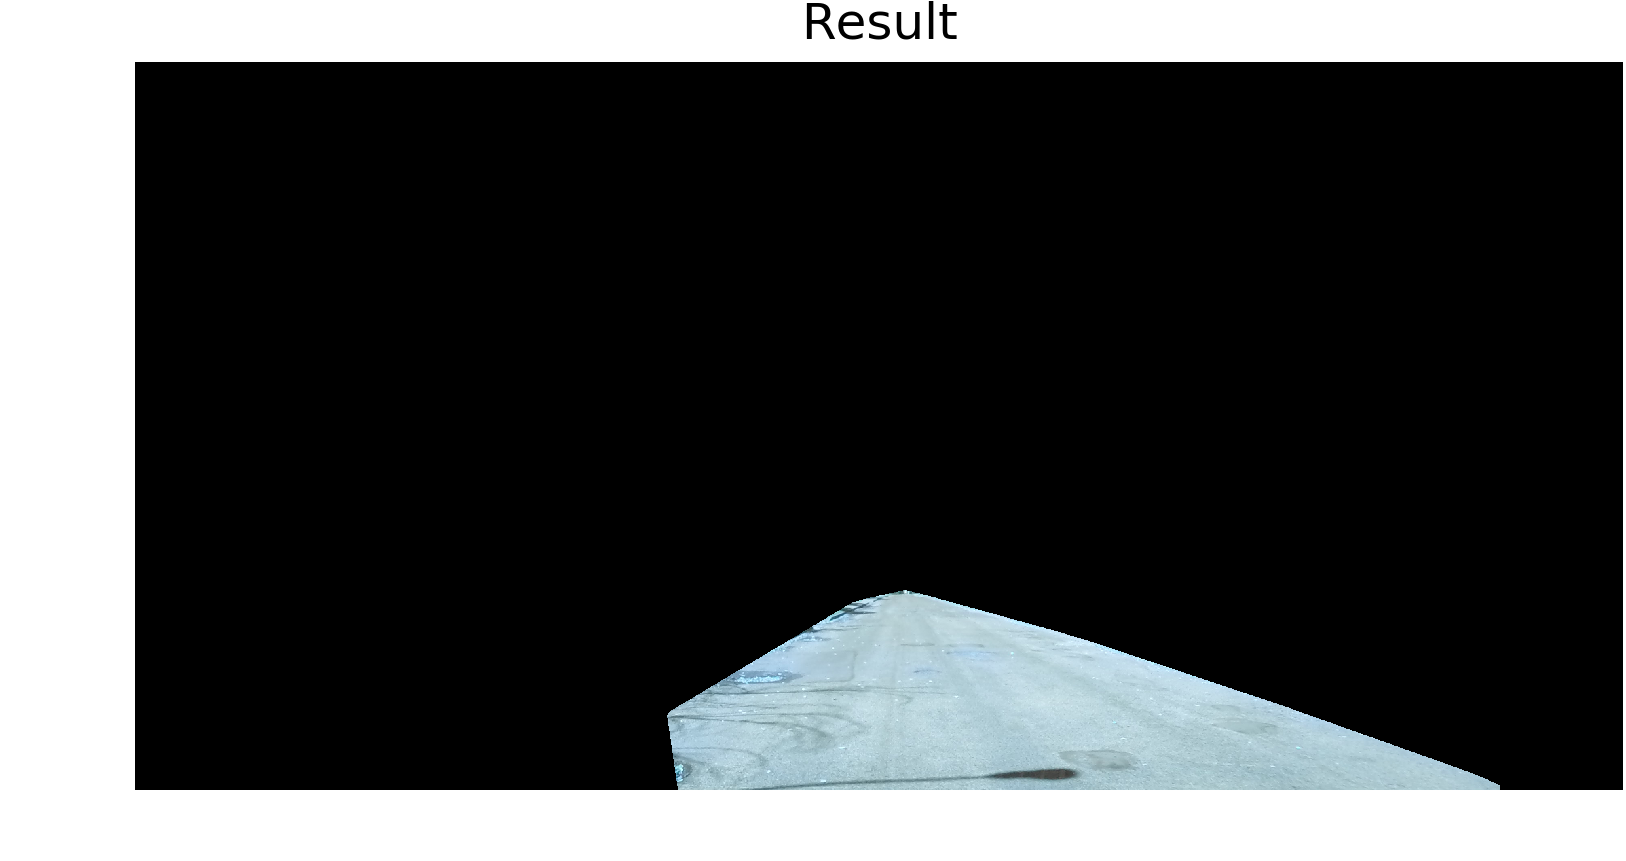
\includegraphics[scale=0.25]{Images/7_Result.png}
\end{center}
\caption{Extracted Road}
\end{figure}


\subsubsection{Blob Detection Method}


\subsection{Machine Learning Techniques}

In this section we describe in details the various machine learning techniques that we used for detecting the presence of the pothole in the roads.

\subsubsection{Feature Modelling}

We used SIFT and SURF detectors to extract feature from the image and train the classifier.

\subsubsection{Machine Learning Algorithms}

\begin{itemize}
\item SVM

\item KNN

\end{itemize}

\section{Results}
We collected a set of images from various lightening conditions for our analysis. The annotation of the potholes has been done manually. The data set is then divided into Positive and Negative samples. 

\subsection{Pothole visualisation using Image processing Techniques}



\subsection{Pothole detection using Machine Learning Techniques}


A table containing the accuracy of the ML techniques that we used.

\section{Conclusion}
The conclusion goes here.


\appendices
\section{Pseudo code for Image processing}
Appendix one text goes here.

% you can choose not to have a title for an appendix
% if you want by leaving the argument blank
\section{Pseudo code for Machine Learning}
Appendix two text goes here.


% use section* for acknowledgment
\section*{Acknowledgment}
We would like to thank Prof. Dinesh Babu Jayagopi for guiding us throughout this venture, Prof. MJ (Thinus) Booysen, Associate Professor at the Electrical $\&$ Electronic Engineering Department at Stellenbosch University for allowing us to use pothole datasets \cite{dataset}.


% Can use something like this to put references on a page
% by themselves when using endfloat and the captionsoff option.
\ifCLASSOPTIONcaptionsoff
  \newpage
\fi

\begin{thebibliography}{1}

\bibitem{paperone} 
S. Nienaber, M.J. Booysen, R.S. Kroon
\textit{Detecting potholes using simple image processing techniques and Real-world Footage, 2015}. 
SATC, July 2015, Pretoria, South Africa
\url{http://scholar.sun.ac.za/handle/10019.1/97191}
 
\bibitem{papertwo} 
Ajit Danti, Jyoti Y. Kulkarni, and P. S. Hiremath, Member, IACSIT
\textit{An Image Processing Approach to Detect Lanes, Pot Holes and Recognize Road Signs in Indian Roads, December 2012}
\url{http://www.ijmo.org/papers/204-S3015.pdf}

\bibitem{paperthree}
S. Nienaber, R.S. Kroon, M.J. Booysen  
\textit{“A Comparison of Low-Cost Monocular Vision Techniques for Pothole Distance Estimation”}
IEEE CIVTS, December 2015, Cape Town, South Africa.
 
\bibitem{dataset}
The annotated image dataset used in the pothole detection is freely available at
\url{https://goo.gl/3QyeMs}

\bibitem{pothole}
\url{https://en.wikipedia.org/wiki/Pothole}

\end{thebibliography}

\begin{IEEEbiography}[{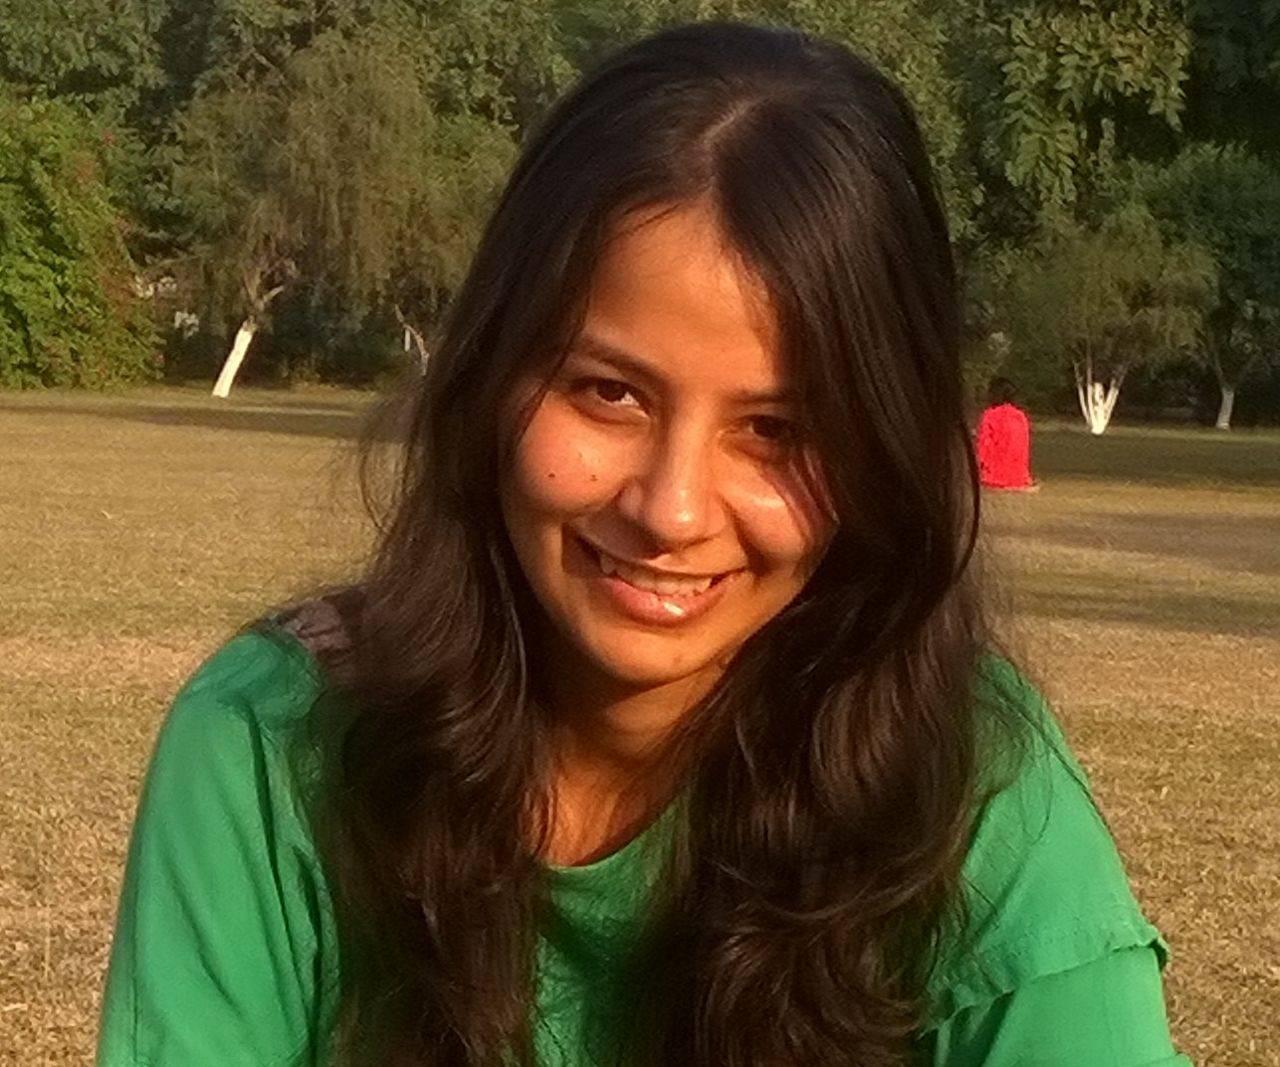
\includegraphics[width=1in,height=1.25in,clip,keepaspectratio]{Images/akanksha.jpg}}]{Akanksha Dwivedi}
is currenlty pursing Master of Technology from International Institute of Information Technology, Bangalore. 
\end{IEEEbiography}

% if you will not have a photo at all:
\begin{IEEEbiography}[{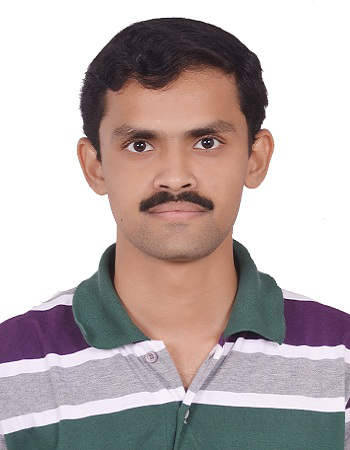
\includegraphics[width=1in,height=1.25in,clip,keepaspectratio]{anoop.jpg}}]{Anoop Toffy}
is currenlty pursing Master of Technology from International Institute of Information Technology, Bangalore. 
\end{IEEEbiography}

% insert where needed to balance the two columns on the last page with
% biographies
%\newpage

\begin{IEEEbiography}[{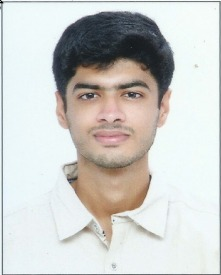
\includegraphics[width=1in,height=1.25in,clip,keepaspectratio]{Images/athul.jpg}}]{Athul Suresh}
is currenlty pursing Master of Technology from International Institute of Information Technology, Bangalore. 
\end{IEEEbiography}

\begin{IEEEbiography}[{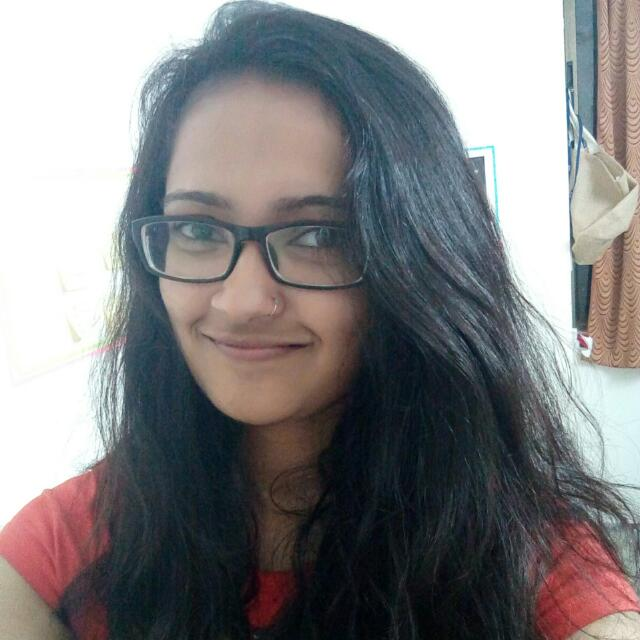
\includegraphics[width=1in,height=1.25in,clip,keepaspectratio]{Images/tarini.jpg}}]{Tarini Chandrashekhar}
is currenlty pursing Master of Technology from International Institute of Information Technology, Bangalore. 

\end{IEEEbiography}

\end{document}


